\chapter{Working with Patches\label{ch:intro_patches}}

\setcounter{section}{-1}

\section{Assigned Readings for the Class Today}

\begin{enumerate}
\item \citet[chapter 2, pages 45--68]{wilensky_rand_2015}
\item {\it NetLogo User Manual} (\url{http://ccl.northwestern.edu/netlogo/docs/} and installed on
  your computer
  with the NetLogo distribution):
\begin{itemize}
\item Tutorial \#1: Models
\item Tutorial \#2: Commands
\item Tutorial \#3: Procedures
\end{itemize}
And the NetLogo program Life Simple, found in the Models Library, {\it IAMB Textbook} folder, in the {\it chapter 2} folder.
\end{enumerate}



\section{Crib Sheet}

\subsection{Navigating NetLogo}
\begin{enumerate}
\item Three tabs: Interface, Info, Code. 
\item In the Code tab, our first \emph{procedure}, a \emph{command procedure}.
\begin{verbatim}
to hello-world
  print "Hello, world!"
end
\end{verbatim}
Points arising:
\begin{enumerate}
\item General pattern for a command procedure in NetLogo:
\begin{verbatim}
to <command name>
     <Block of one or more lines of code.>
end
\end{verbatim}
\item \verb+< ... >+ is markup indicating that you the programmer need to substitute in appropriate NetLogo expressions or lines of code.
\item Sequences of characters---called \emph{strings}---are indicated by opening and closing double quotes.
\item \verb+print <expression>+ prints the expression to the the Command Center window on the Interface tab.
\end{enumerate}
\item NetLogo programs are built with procedures. There are two kinds: command procedures and reporters. Both are put into the Code tab, which is a text editor aware of the NetLogo programming language. We'll discuss reporters later.
\item Normally, NetLogo programs will have a procedure called \texttt{setup} and a procedure called \texttt{go}. This is conventional and appropriate but hardly required.
\item User interface widgets: creating with point-and-click.

Create a button that \emph{calls} the \texttt{hello-world} procedure. Click on it. What happens?

\item Menu items and help.
\item Inspecting patches.

See Figure \ref{fig:inspect_patch}. What happens if you edit the properties?



 \begin{figure}[htbp] %  figure placement: here, top, bottom, or page
    \centering
    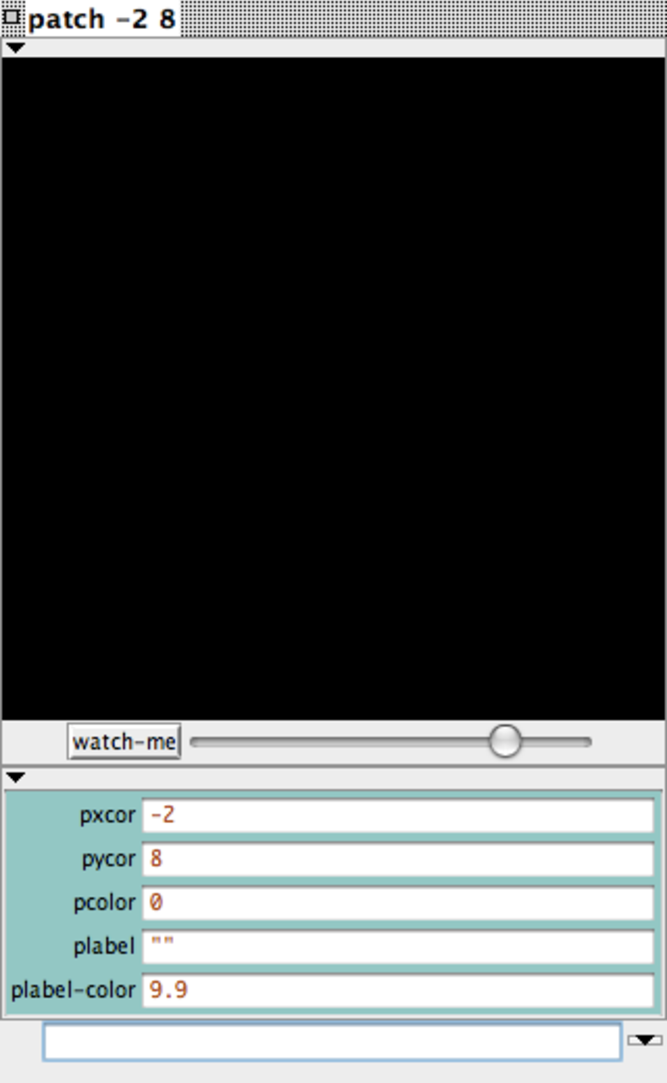
\includegraphics[width=3in]{figures/inspect-patch.pdf}  
    \caption{Inspecting a patch with default settings.} 
    \label{fig:inspect_patch}
 \end{figure}

\item Inspecting turtles.

See Figure \ref{fig:inspect_turtle}. What happens if you edit the properties?

 \begin{figure}[htbp] %  figure placement: here, top, bottom, or page
    \centering
    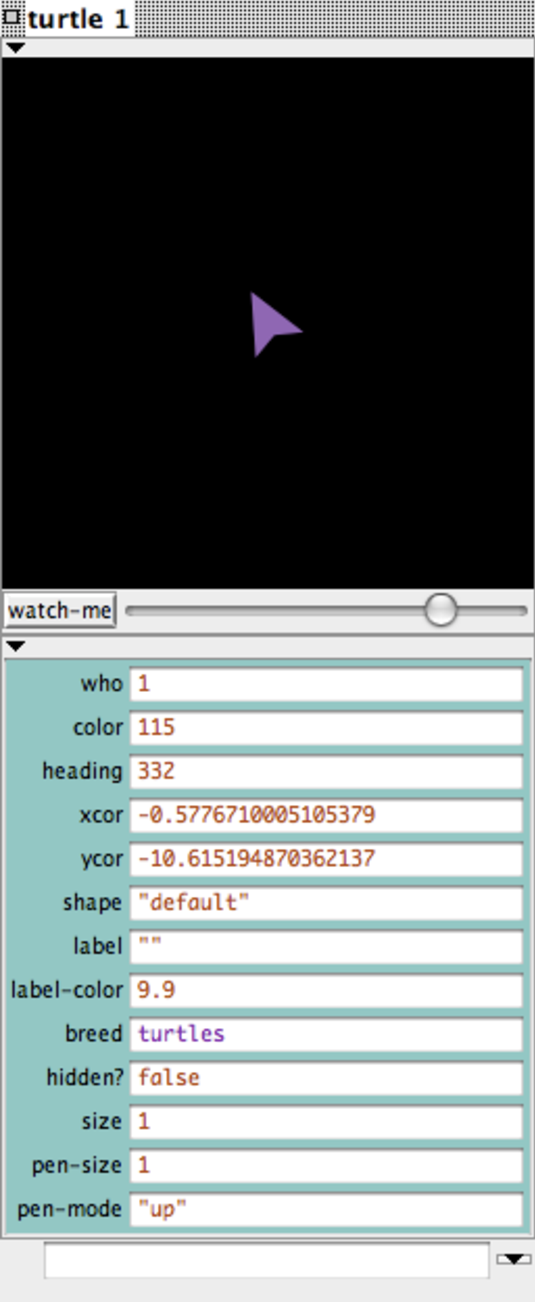
\includegraphics[width=3in]{figures/inspect-turtle.pdf}  
    \caption{Inspecting a turtle with default settings.} 
    \label{fig:inspect_turtle}
 \end{figure}

\item NetLogo is \emph{not} case sensitive.
\end{enumerate}

\clearpage\newpage
\subsection{The Game of Life}

\subsection{Coding points}

To begin, see the readings for today in our textbook: \citet[chapter 2, pages 45--68]{wilensky_rand_2015}. We'll begin with the code on page 51.

\begin{enumerate}
\item Here is the \texttt{setup} command procedure in the Life Simple model:
\begin{verbatim}
to setup
  clear-all
  ask patches
  ;; create approximately 10% alive patches
    [ 
      set pcolor blue - 3 ;; dark blue cells are dead
      if random 100 < 10 
      [ set pcolor green ] ;; green cells are alive
    ]
    reset-ticks
end
\end{verbatim}
Notice that it fits the command procedure pattern discussed above. Now, let's look into it.

\item \verb+clear-all+ is normally the first line of the \texttt{setup} procedure. It resets/clears everything that can be reset/cleared.

\item \begin{verbatim}
ask patches [<Block of one or more lines of code.>]
\end{verbatim}
Creates a patch context inside the square brackets, randomly orders the patches and then sequentially executes the\newline
 \verb+<Block of one or more lines of code.>+ \newline on each patch.

\item \texttt{ask} is a very important command in NetLogo. See the ``ask'' section in the NetLogo  ``Programming Guide''. It's what you use to get agents to do things. Patches are agents in NetLogo. So are turtles and links. All in due time.
\item The square brackets after \texttt{ask patches}, \verb+[ ... ]+, are necessary, but their placement is quite flexible. Put them as you will for the sake of clarity. The book's example is a good one.

\item  \texttt{ask patches} is said to create a \emph{patch context} within the square brackets. In this context, commands are automatically addressed to patches. You can think of it this way. When  \texttt{ask patches} is executed, NetLogo makes a randomized list of patches. It does this each time  \texttt{ask patches} is executed, so that it processes the commands on the patches in a different, random order each time. Then, having created the randomized list, NetLogo processes the commands on one patch at a time, using the order indicated in the randomized list.
\item \texttt{set pcolor blue} This is a deceptively simple command. Understand how it works and you will understand a lot about how NetLogo works.  \texttt{pcolor} is a patch attribute or property; it comes with every individual patch. See Figure \ref{fig:inspect_patch}.  

\item \texttt{blue} is a NetLogo built-in constant, used for indicating a certain shade of \ldots blue!  Try typing \texttt{blue} Command Center (at the \verb+observer>+ prompt. What do you get?

\item \texttt{set} is NetLogo's command for assigning a value to a variable. A variable is a symbol whose value can vary, can be changed, so \texttt{pcolor} is a variable that attaches to each patch separately.
The patten is:

\verb+set <variable> <value>+

\noindent with the meaning ``Give the variable \verb+<variable>+ the value \verb+<value>+.'' In other languages this is typically done with something like:

\verb+<variable> = <value>+

\noindent but not in NetLogo.

\item Now an important question: When NetLogo executes \texttt{set pcolor blue} in the above \texttt{setup} procedure, how does it know which patch to set to blue?

Answer: See above for how \texttt{ask} works. NetLogo first makes a random list of the patches, then it works through them one at a time in order. At any given time until the \texttt{ask} task completes NetLogo ``knows'' which patch it is attending to and it executes the commands on that one patch.

\item Execute this procedure a few times to see for yourself:
\begin{verbatim}
to test
  ca
  ask patches 
  [
    set pcolor red
    wait 0.5
  ]
end
\end{verbatim}
(Use Halt under the Tools menu to stop execution of the procedure.)
\item Look up and read about the \texttt{set} command in the ``Programming Guide.''
\item Next we have a \emph{flow control} statement, here an \texttt{if}.
\begin{verbatim}
      if random 100 < 10 
      [ set pcolor green ] ;; green cells are alive
      \end{verbatim}

\item /* here */
\end{enumerate}

\section{For More Information}

/* References on the Game of Life. */


\ifnum\draft=1
\vfill
\noindent\verb+$Id: intro-patches.tex 4955 2015-09-15 21:39:07Z sok $+
\fi